\section{SEGUNDO TEMA}

En esta sección se revisan modelos matemáticos capaces de describir de forma analítica una amplia gama de comportamientos inelásticos complejos presentes en muchos sistemas y materiales.

	\subsection{Modelo Histerético de Bouc-Wen} \label{subsection:MHBW}
	
Es un modelo que se usa para predecir el comportamiento dinámico no lineal de aisladores sísmicos, así como de disipadores histeréticos. El modelo de Bouc-Wen necesita cuatro parámetros de entrada, los cuales son: la rigidez elástica, la rigidez postfluencia, la fuerza característica y un parámetro adimensional que controla la forma del lazo histerético.

De acuerdo con \citet{Charalampakis2010} la fuerza en el tiempo \textit{t} del modelo histerético de Bouc-Wen se evalúa en función del desplazamiento de la siguiente manera:
\begin{gather}
F(t)=\alpha \frac{F_{y}}{D_{y}}u(t)+(1-\alpha)F_{y}z(t)				\label{BoucWen1} \\
\begin{aligned}
\dot{z}(t)=\left[1-\left|z(t)\right |^{\eta}sgn(\dot{u}(t)z(t))\right]\frac{\dot{u}(t)}{D_{y}}&,&\hspace{1em}& z(0)=0 \\
\end{aligned}		\label{BoucWen2}
\end{gather}

	\begin{figure}[!h]
	\centering
		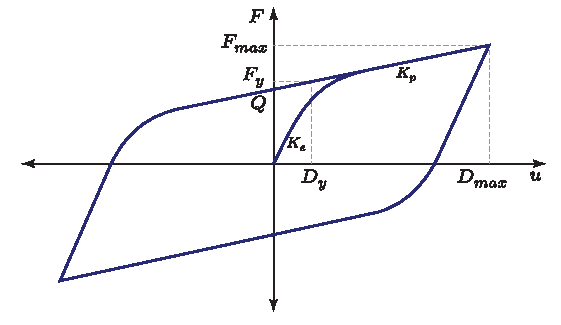
\includegraphics[scale=1]{E_IMAGENES/1_Capitulo2/Cap2_Imagen6.pdf}
		%\vspace{-3 mm}
	\caption[Modelo histerético de Bouc-Wen]{\centering\footnotesize Modelo histerético de Bouc-Wen. Adaptado de \citet{Charalampakis2010}}
	\label{Cap2_Figura6}
	\end{figure}

En la \autoref{Cap2_Figura6} y en las ecuaciones \ref{BoucWen1} y \ref{BoucWen2} se muestran los parámetros necesarios para definir un ciclo histerético con comportamiento de Bouc-Wen.

Donde:

%Inicar tabla explicando cada Parámetro
\begin{tabular}{L{0.5 cm}p{0.025 cm}p{11.5 cm}}
  $K_{e}$ & : & Rigidez elástica \\
  $K_{p}$ & : & Rigidez postfluencia \\
  $Q$     & : & Fuerza característica \\
  $D_{y}$ & : & Desplazamiento de fluencia \\
  $F_{y}$ & : & Fuerza de fluencia \\
  $\alpha$ & : & Razón entre la rigidez postfluencia y la rigidez elástica  \\
  $\eta$ & : & Parámetro adimensional que controla la forma del lazo histerético \\
 \end{tabular}\\

	
 
 